\documentclass[a4paper, 11pt]{article}

\usepackage[utf8]{inputenc}
\usepackage{graphicx}
\usepackage[francais]{babel}
\usepackage{authblk}
\usepackage{hyperref}
\usepackage{subfigure}
\title{Une (trop) rapide introduction a Qgis}
\author[123]{Etienne Delay}
\affil[1]{1 CIRAD UPR GREEN, F-34398 Montpellier, France}
\affil[2]{GREEN, CIRAD, Univ. Montpellier, Montpellier France}
\affil[3]{Laboratoire GEOLAB UMR 6042 CNRS, Universit\'e de Limoges, FLSH. 39E rue Camille Gu\'erin, 87036 Limoges, France}
%\date{}       %% if you don't need date to appear
\begin{document}

\maketitle
Ce document est disponible sur github\footnote{Lien vers les sources du document : \url{https://github.com/ElCep/introductionSIG_osgeo}, consulté le 14 janvier 2019}
\section{Installation de Qgis}
  Qgis est devenu ces dernières années l'outil libre (sous licence GNU-GPL) le plus polyvalent en cartographie interfacer avec par exemple GRASS-GIS et SAGA-GIS qui sont des librairies de calcul très puissantes sur des rasters, ou encore la possibilité de se connecter à des bases de données relationnelles (postgreSQL-postgis, oracle, ...).

  La grande nouveauté est également dans le portage de Qgis vers une solution serveur (ce qui veut dire que vous pourrez facilement créer des cartes dynamiques en ligne, pour peu que vous ayez un serveur), le développement d'une solution légère de consultation (qgis browser), et d'une version androïd !

  Pour travailler, vous commencerez donc par installer Qgis sur votre machine. Le type d'installation va dépendre du système d'exploitation que vous avez sur votre machine.

  Pour Linux c'est le plus facile (distributions Fedora, Ubuntu, debian, openSuse, Rhel, CebtOS, Scientific Linux, Mandriva, Archlinux), des packages sont disponibles dans vos dépôts et vous pouvez suivre les instructions.

  Pour Mac, KyngChaos (un gentil contributeur) à longtemps fournis les sources compiler, mais aujourd'hui pour la version OS 10.11 (El Capitain et plus récent) vous pouvez télécharger un fichier.dmg directement sur le site de QGis en suivant scrupuleusement les informations contenues dans le Read Me sur le disque image.

  Pour Windows, vous devez choisir l'architecture de votre processeur (32 bit ou 64 bit), mais pas de crainte, si vous ne téléchargez pas le bon, il ne s'installera pas. Je vous conseille plus que vivement d'utiliser l'installateur OSGeo4W (OSgeo for Windows) qui va vous permettre d'installer davantage de dépenses. Cependant, dans certaines situations, vous ne pourrez installer Qgis qu'avec l'installateur indépendant... donc il faudra expérimenter!

\section{Premiers contacts}
  \subsection{Qgis un logiciel incuber par l'OSGeo}

  \subsection{Quoi de neuf dans Qgis3}
  QGis 3\footnote{La présentation de Jean-Marie Arsac aux rencontres QGIS 2017 a servi de base à cette section. Vous pouvez retrouver la présentation sur github : \url{https://github.com/OSGeo-fr/QGIS-user-fr/blob/master/2017/presentations/01_matin/01_Azimuth_nouveautes_QGIS_3.pdf}, consulté le 15 janvier 2018} est une réécriture complète du logiciel passant ainsi de Pyhton2\footnote{Qgis utilisait notement Python 2.7.5-2 qui n'avait pas évolué depuis 2010} à Python3 et de Qt4\footnote{Qt4 était problématique sur MacOS et les dériver de Debian, tendis que Qt5 est bien mieux supporté et tire parti des écrans rétina, et support la mobilité} à Qt5. Cette rupture était nécessaire, car ces deux librairies étaient vieillissantes et menacées de ne plus être maintenues sur un grand nombre de systèmes.

  Aujourd’hui, dans la version LTR\footnote{Vous pouvez jeter un coup d'oeil sur la Road Map du projet QGIS : \url{https://www.qgis.org/en/site/getinvolved/development/roadmap.html} consulté le 15 janvier.} (\textit{long-term release}) est la version 3.4 si un grand nombre d'extensions ont été portées dans la nouvelle API, la majorité est restée bloquer en 2.X.

  Mais remettre à plat le code en passant à Python3 voulait dire remettre aussi à plat l'API (\textit{application programming interface}) et potentiellement casser toutes les extensions. Or Qgis avec les années est devenu LA porte d'entrée sur une constellation d'outils de traitement de données géospatiales donc le danger de rompre la communauté était grand.

  On notera des nouveautés dans l'interface (fig. \ref{fig:qgis3-interfaces}), mais également dans le coeur du logiciel, refactoring du C\#, un éditeur de \textit{Dublin core}, l'intégration de GeoNode. Le composeur d'impression a été ré écrit pour mieux gérer la mise en page (nouveaux symbole, nouveaux algorithmes de coloriage, de non-chevauchement).

  Pour l'interface avec les bases de données, postgreSQL et SQLite sont très bien supporté (avec des request de mise-a-jour régulières). Enfin je voulais attirer votre attention sur un nouveau format par défaut baptisé GPKG qui vise à s'extraire du format \textit{legacy} ESRI qu'est le \textit{shapefile}.
  \begin{figure} %%%script issu de script/map_surfaces_viticole_mondiale.R
  \centering
    \subfigure[]{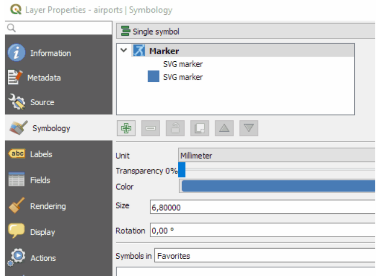
\includegraphics[width=0.45\textwidth]{img/interface_qgis1}\label{fig:qgis31}}
    \subfigure[]{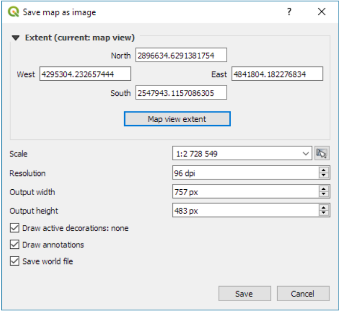
\includegraphics[width=0.45\textwidth]{img/interface_qgis2}\label{fig:qgis32}}\\
    \subfigure[]{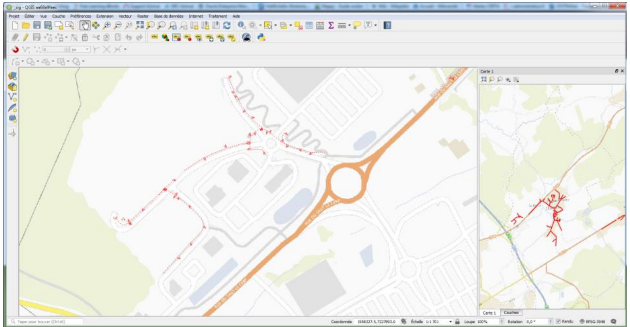
\includegraphics[width=0.9\textwidth]{img/interface_qgis3}\label{fig:qgis33}}
    \subfigure[]{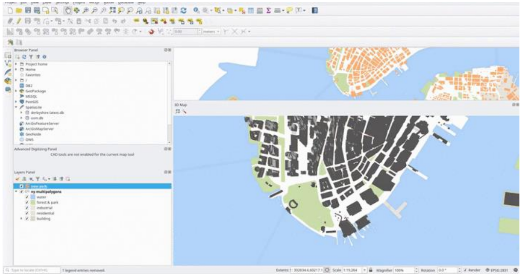
\includegraphics[width=0.9\textwidth]{img/interface_qgis4}\label{fig:qgis34}}
    \caption{Quelques capuces de l'interface de QGIS3. Sur la figure \subref{fig:qgis31} on constate l'ajout d'une barre de recherche dans les propriétés de la couche, en
     \subref{fig:qgis32} la possibilité d'exporter la carte rapidement sans passer par le composeur d'impression, \subref{fig:qgis33} Le support du multi-point-de-vue et
     \subref{fig:qgis34} le support de la 3D}
    \label{fig:qgis3-interfaces}
  \end{figure}

  \subsection{Quelles données sont lisibles?}
  Vous pouvez afficher et superposer des couches de données rasters et vecteurs dans différents formats et projections sans avoir à faire de conversion dans un format commun. Les formats supportés incluent :
  \begin{itemize}
    \item les tables spatiales et les vues PostGIS,SpatiaLite, MSSQL Spatial et Oracle Spatial, les formats vecteurs supportés par la bibliothèque OGR installée, ce qui inclut les Shapefiles ESRI , MapInfo, SDTS, GML et beaucoup d’autres, voir section les données vectorielles.
    \item les formats raster supportés par la bibliothèque GDAL (Geospatial Data Abstraction Library) tels que GeoTiff, Erdas img., ArcInfo ascii grid, JPEG, PNG et beaucoup d’autres, voir section Les données raster.
    \item les outils de Traitements QGIS pour lancer, depuis QGIS, des centaines d’algorithmes natifs ou provenant d’applications tierces, voir section Introduction du chapitre sur les Outils de traitements.
    \item les formats raster et vecteurs provenant des bases de données GRASS.
    \item les données spatiales provenant des services réseaux OGC comme le WMS, WMTS, WCS, WFS, WFS-T, etc.
    \item les données OpenStreetMap.
  \end{itemize}
  \subsection{Charger et afficher les couches raster ou vecteur depuis le jeu de données test}

  \begin{itemize}
    \item Cliquez sur l’icône gestionnaire des sources open-data (CTRL+L) 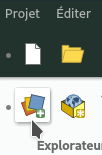
\includegraphics[width=1.5cm]{img/qgis_gestionnaire_de_sources}.
    \item La boite de dialogue s'ouvre (fig \ref{fig:boiteDialogueSource}) et vous permet de choisir le type de données à ouvrir. Pour les données vecteur et raster  "Fichier" devrait être sélectionnés comme Type de source dans la fenêtre. Vous pouvez inscrire le chemin dans le menu ou utiliser le bouton \texttt{...} pour parcourir l'arborescence.
    \item Parcourez le dossier où vous avez téléchargé les données du cour, sélectionnez le fichier "departement\_geofla" et cliquez sur [Ouvrir], et enfin, dans la boîte de dialogue Ajouter une couche vecteur, cliquez sur [OK].
    \item Zoomez sur une zone de votre choix (molette de la souris ou outils de zoom).
    \item Double-cliquez sur la couche \texttt{departement\_geofla} dans la liste des couches pour ouvrir la fenêtre; ou click droit et Propriété des couches (fig. \ref{fig:boiteDialoguePropriete}).
    \item Cliquez sur l’onglet Style et sélectionnez le bleu comme couleur de remplissage.
    \item Cliquez sur l’onglet Étiquettes et sélectionnez \texttt{étiquettes simples}(fig. \ref{fig:boiteDialogueEtiquette}) pour permettre l’étiquetage des entités. Choisissez le champ intitulé NOM\_DEP comme champ d’étiquetage.
    \item Pour améliorer la lisibilité des étiquettes, vous pouvez ajouter un halo autour d’elles, en cliquant sur “Tampon” dans la liste à gauche puis sur checkbox Affiche un tampon. Choisissez 3 comme taille du tampon.
    Cliquez sur \texttt{[Appliquez]} pour vérifier si le résultat est satisfaisant et enfin cliquez sur \texttt{[OK]}.
  \end{itemize}

  \begin{figure}
  \centering
    \subfigure[]{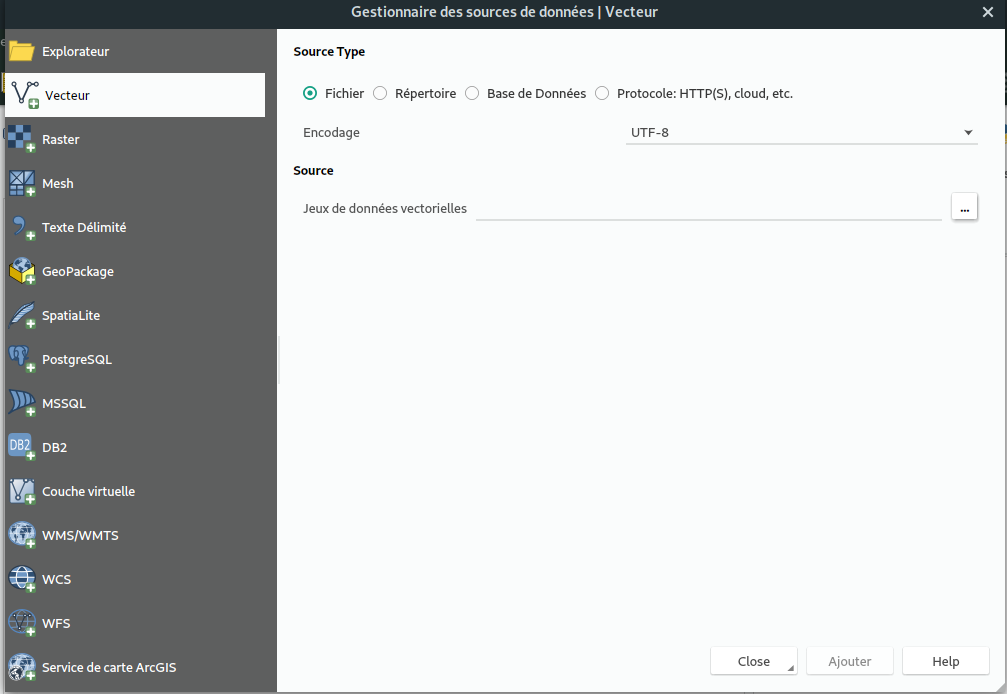
\includegraphics[width=0.45\textwidth]{img/bd_sources}\label{fig:boiteDialogueSource}}
    \subfigure[]{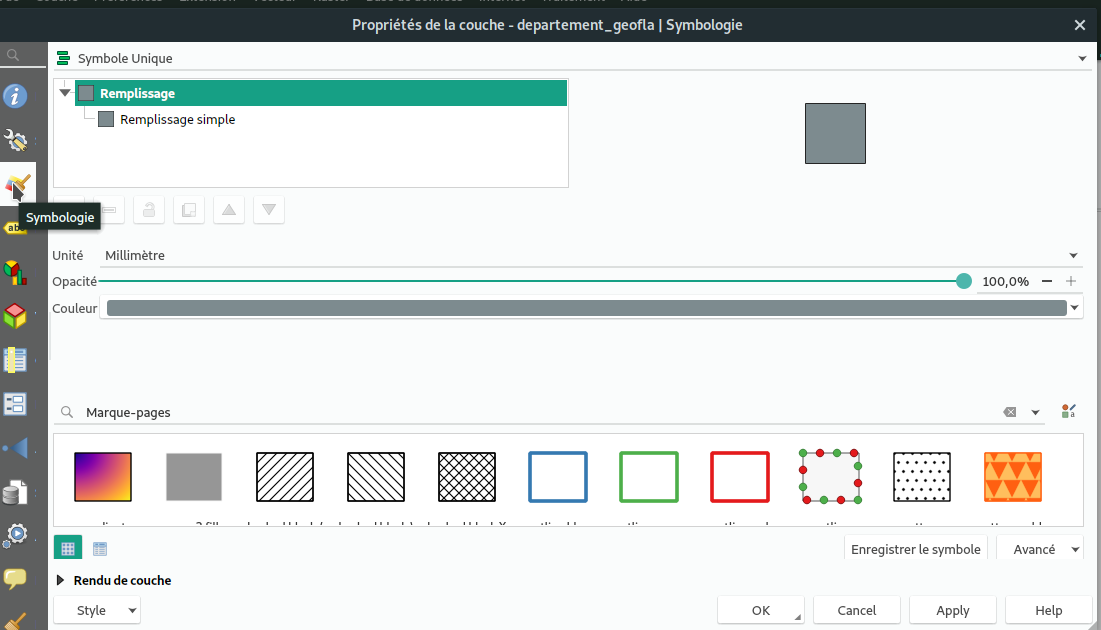
\includegraphics[width=0.45\textwidth]{img/bd_proprieteCOuche}\label{fig:boiteDialoguePropriete}}\\
    \subfigure[]{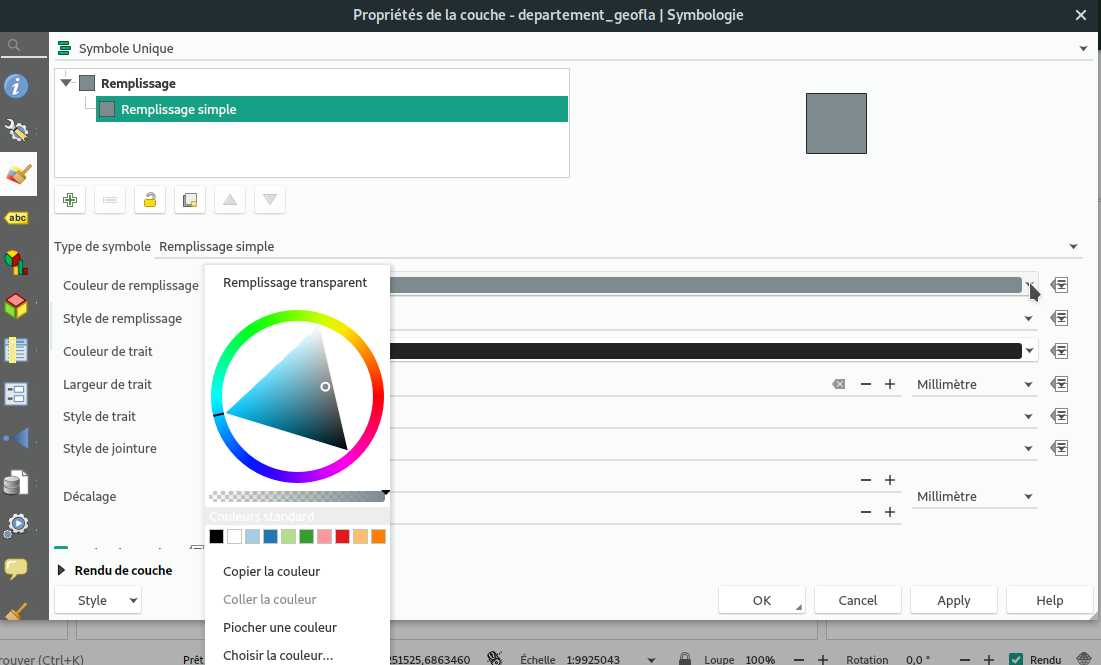
\includegraphics[width=0.45\textwidth]{img/bd_remplissage}\label{fig:boiteDialogueRemplissage}}
    \subfigure[]{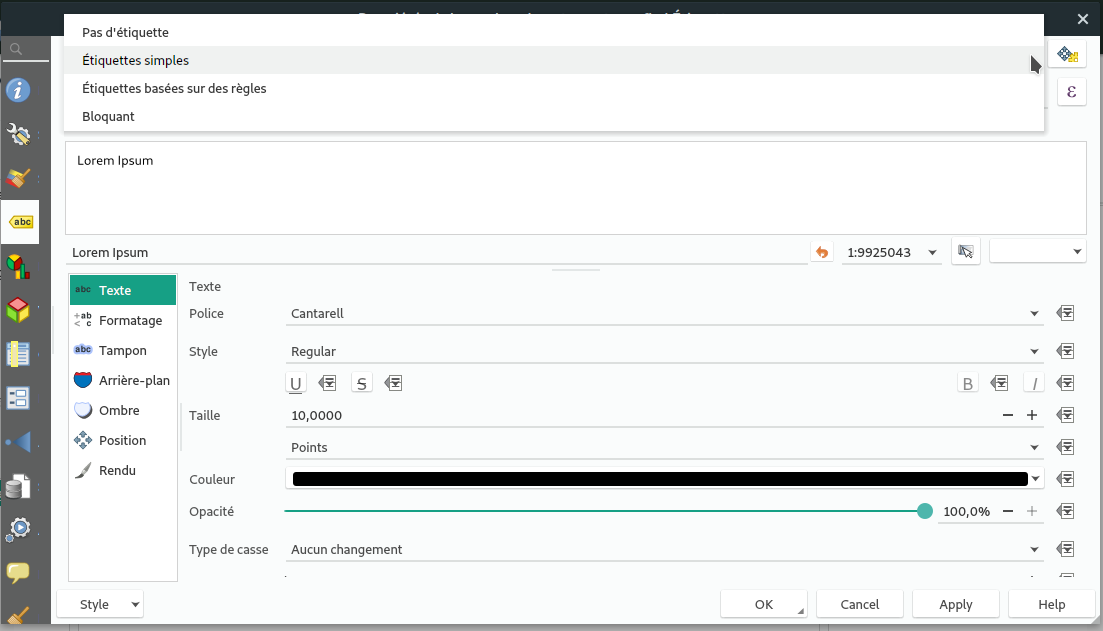
\includegraphics[width=0.45\textwidth]{img/bd_etiquette}\label{fig:boiteDialogueEtiquette}}
    \caption{Les boites de dialogues. \subref{fig:boiteDialogueSource} pour ajouter une couche, pour modifier les propriétés de la couche \subref{fig:boiteDialoguePropriete}, \subref{fig:boiteDialogueRemplissage}, et les étiquette \subref{fig:boiteDialogueEtiquette}}
    \label{fig:qgis3-dialogues1}
  \end{figure}

Pour charger des couches raster vous utiliserez le bouton couche raster, la démarche est relativement similaire.

Vous pouvez constater combien il est facile d’afficher des couches dans QGIS. La carte produite est loin d'être belle, mais tout fonctionne (fig. \ref{fig:carte1})!

\begin{figure}
\centering
  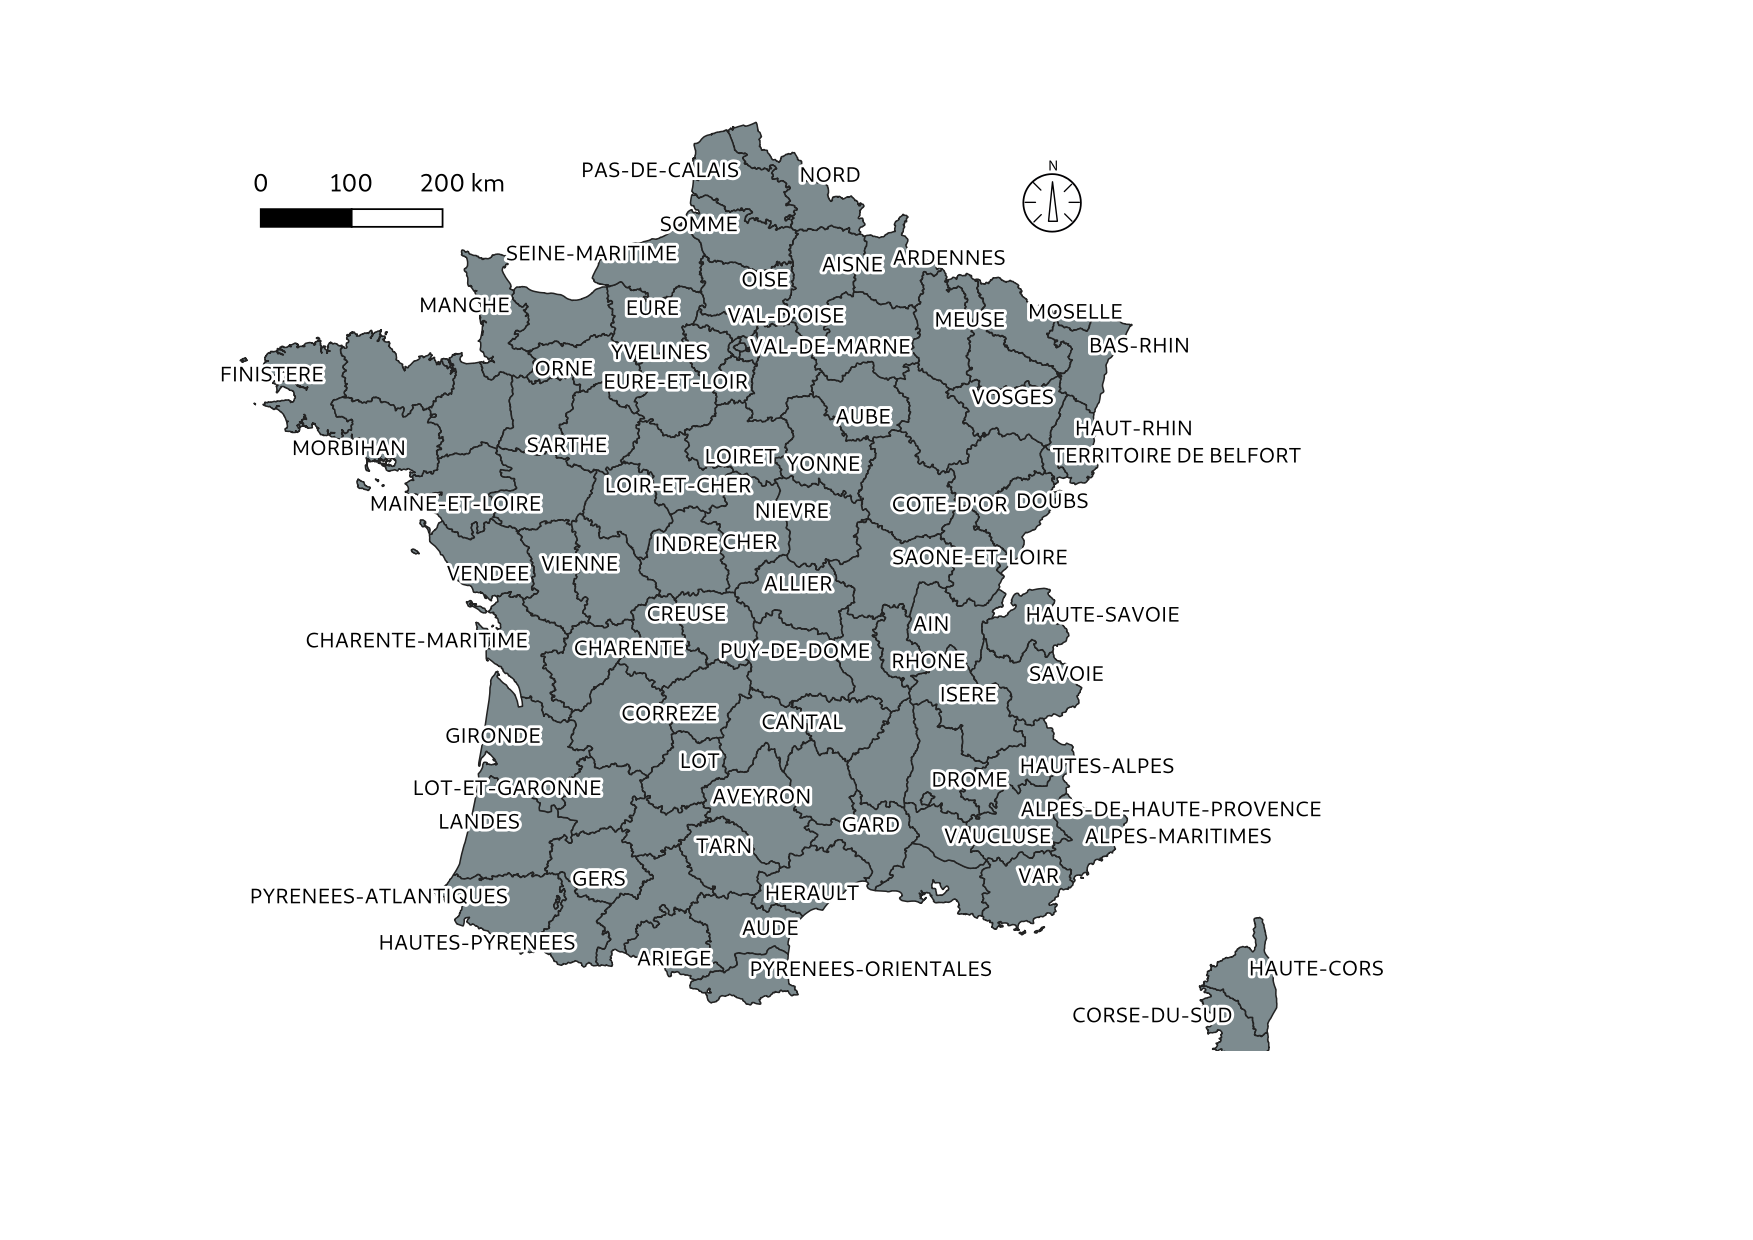
\includegraphics[width=0.9\textwidth]{img/carte_france1}
  \caption{Une première carte de France}\label{fig:carte1}
\end{figure}

\section{Ma première analyse thématique}
Le minimum que l'on demande à un outil de géomatique est de faire des analyses thématiques. En repartant du travail que vous avez effectué à la couche précédente, nous vous proposons donc deux choses :
  \begin{itemize}
    \item intégrer de nouvelles données "intéressantes" à cette couche avec une belle jointure de table.
    \item faire une analyse thématique sur ces données nouvellement intégrées.
  \end{itemize}

  \subsection{Analyse thématique}
  \subsubsection{Importer des données non géographiques}\label{part:chargerData}
  Pour effectuer une jointure de table dans Qgis, il faut dans un premier temps ouvrir la couche vectorielle (nous garderons ici les départements de la base geofla de l'IGN qui sous "licence ouverte" version 1.0 ), puis, de la même manière qu'on ouvre une couche vectorielle, on peut ouvrir une table de données (csv, odb, xls) en prenant soin de rendre visible tout les fichiers dans la fenêtre de sélection. Vous avez un fichier CSV, vous pouvez choisir le "Texte Délimité" pour le charger en temps que table. Comme c'est une couche sans géométrie (comprendre de la donnée textuelle sans lien spatial), il faudra le spécifier dans \texttt{Définition de la géométrie}.

  \begin{figure}
  \centering
    \subfigure[]{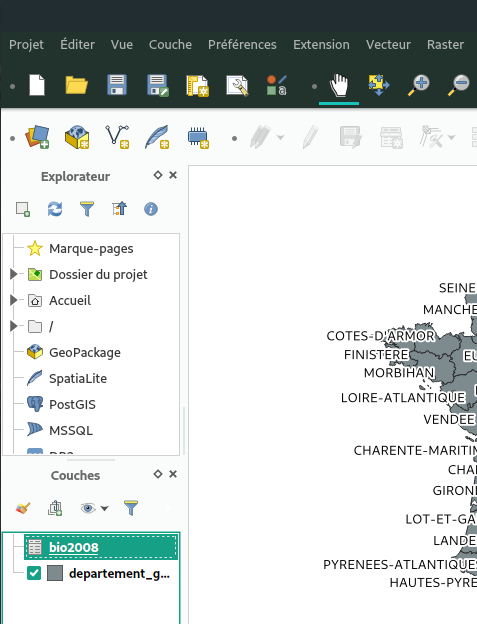
\includegraphics[width=0.2\textwidth]{img/gestionnaire_de_couches}\label{fig:interfaceCouches}}
    \subfigure[]{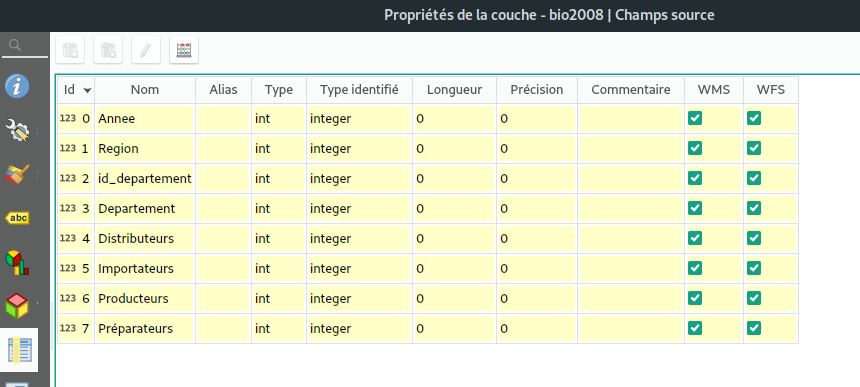
\includegraphics[width=0.8\textwidth]{img/prop_table}\label{fig:boiteDialogueProprieteTable}}\\
    \subfigure[]{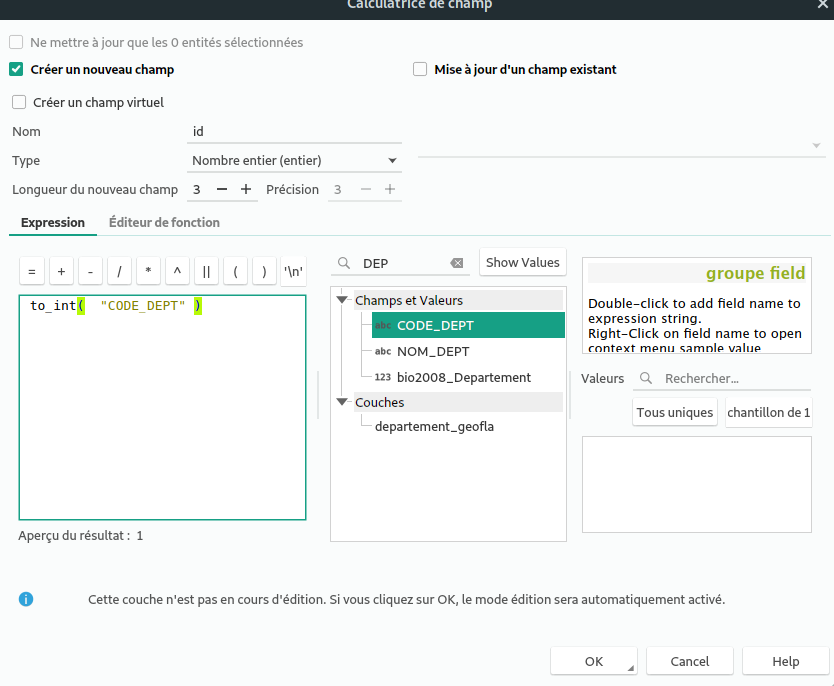
\includegraphics[width=0.6\textwidth]{img/convertion_int}\label{fig:converttion_int}}
    \subfigure[]{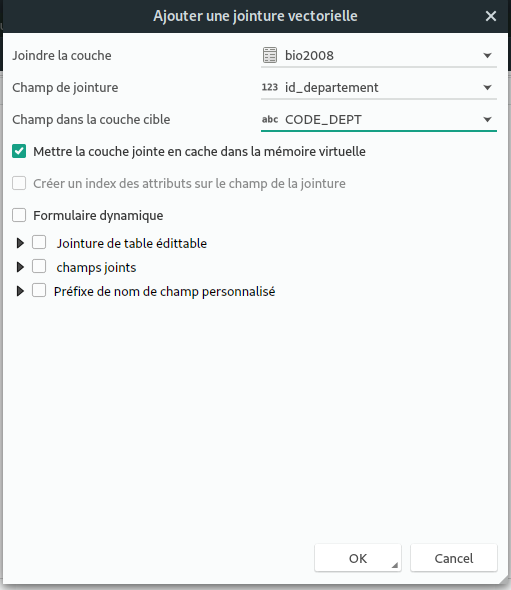
\includegraphics[width=0.4\textwidth]{img/bd_jointure}\label{fig:boiteDialoguejointure}}
    \caption{Les boites de dialogues. \subref{fig:boiteDialogueSource} pour ajouter une couche, pour modifier les propriétés de la couche \subref{fig:boiteDialoguePropriete}, \subref{fig:boiteDialogueRemplissage}, et les étiquette \subref{fig:boiteDialogueEtiquette}}
    \label{fig:qgis3-dialogues1}
  \end{figure}

  Les deux documents apparaissent en temps que couche dans l'interface prévue à cet effet (fig. \ref{fig:interfaceCouches}). Il faut maintenant vérifier que vous avez deux tables qui seront assemblables (fig. \ref{fig:boiteDialogueProprieteTable}). Pour cela, outre le fait d'avoir une colonne similaire (ce qui est le minimum quand on cherche à joindre deux tables), il faut vérifier que le champ à assembler est bien de la même nature (on cherchera à avoir des caractères avec des caractères, des entiers avec des entiers, des numériques avec des numériques...). On accède à cette donnée dans les propriétés de la couche (fig. \ref{fig:qgis3-dialogues1}).

  On a accès à la nature de la couche en double-cliquant sur celle-ci (ou en effectuant un clic droit et sélectionnant "propriété de la couche"), et en se rendant dans le menu "champs". Pour la couche \texttt{bio2008} on voit donc que tous les champs sont considérés comme des entiers.
  La même vérification pour la couche "département\_geofla" nous montre que la colonne sur laquelle on veut effectuer la jointure est une chaîne de caractères (string). Il faut donc la convertir pour plus de sécurité. C'est ce que nous ferons dans la section suivante.

  \subsubsection{modifier/mettre à jour un champ de la table attributaire}

  La modification d'un champ se fait en ouvrant la table attributaire 
\includegraphics[width=0.5cm]{img/mActionOpenTable} de la couche \texttt{département\_geofla}
et en la rendant modifiable avec 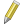
\includegraphics[width=0.5cm]{img/mActionToggleEditing}. Vous allez ensuite utiliser la calculatrice de champs 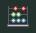
\includegraphics[width=0.5cm]{img/calcul_champ}.

  Vous pouvez alors créer un nouveau champ en remplissant son nom et définissant son type, sa longueur et sa précision.

  Il faudra ensuite définir l'opération à effectuer sur ce champ. Cela s'effectue dans la partie basse de la fenêtre (partie "Expression"). Vous pouvez alors inscrire directement la requête si vous connaissez la syntaxe ou bien vous appuyez sur la liste des fonctions juste au-dessus, en vous aidant de la liste des opérateurs ... (fig. \ref{fig:converttion_int})

  Vous pouvez ensuite valider avec OK et revenir à l'interface de la carte.

  Vous noterez qu'il y a une erreur due à la présence des 2 départements de Corse qui sont A1 et A2. Vous devez supprimer la Corse de la carte (nous n'en aurons pas besoin), ou modifier les code\_dep et les transformer en chiffre (par exemple 999).

  Pour supprimer la Corse, il faut :

  Rester en mode édition de la carte 
\includegraphics[width=0.5cm]{img/mActionOpenTable}  sélectionner les deux départements en avec l’outil  sélection 
\includegraphics[width=0.5cm]{img/mActionSelectRectangle}, en maintenant la touche "Shift" enfoncée, puis en cliquant sur les deux départements de Corse. Ils deviennent alors jaunes. Vous pouvez les supprimer avec 
\includegraphics[width=0.5cm]{img/mActionDeleteSelected}. Vous pouvez recommencer l'étape précédente :-) .

  Il faut maintenant enregistrer votre travail. Vous pouvez soit sauvegarder les modifications sur la couche departement\_geofla, soit faire une sauvegarde sous un autre nom et ainsi conserver la couche initiale propre.

  L'enregistrement de la couche s'effectue en faisant un clic droit sur la couche et en sélectionnant sauvegarder.

  \subsubsection{La jointure en elle même}

  Pour faire une jointure, vous allez dans les propriétés de la couche spatiale dans laquelle vous voulez importer des données, et dans le menu jointure, vous cliquez sur le "+" en bas de la fenêtre. Vous pouvez alors renseigner les couches à joindre et les champs sur lesquels faire la jointure. Dans cet exemple, vous joignez la couche "bio2008" sur le champ "id\_departement" avec le champ que vous avez créé à l'étape (fig. \ref{fig:boiteDialoguejointure}).

  \subsubsection{L'analyse thématique}
  Une fois la jointure effectuée, on va faire immédiatement une analyse thématique sur les données que nous venons de joindre. Vous pourrez faire une analyse thématique très simplement si vous avez normalisé les données de la table attributaire (par exemple en travaillant sur des proportions).

  Mais comme nous sommes sur des valeurs absolues, et que Bertin est un type bien, il faudrait utiliser des symboles proportionnels à la valeur quantitative absolue.

  Pour ça, il faut aller dans les propriétés de la couche, puis dans "Style". Là on peut ajouter un symbole avec le "+" en bas de la fenêtre et choisir remplissage de centroïde. Cela fait apparaitre des points rouges dans la partie couche de symbole. Vous sélectionnez "Marker", symbole simple.

  Là, vous voulez définir une taille proportionnelle. Pour cela vous allez cocher la box en face de "Taille" et modifier le menu en cliquant sur les "..." . Cela va permettre de rentrer une fonction pour les tailles proportionnelles. Vous pouvez alors directement effectuer des opérations sur le champ.

  Vous allez transformer la valeur du champ \texttt{bio2008\_Producteurs} en entier (par sécurité) avec l'expression \texttt{to\_int("bio2008\_Producteurs")}
  puis Ok pour valider (fig \ref{fig:symbolesProp}).

  Astuce : il peut y avoir quelques conflits entre les polygones des départements et les cercles proportionnels. Afin d'éviter cela vous pouvez rendre transparent le remplissage des polygones de cette couche et ouvrir une nouvelle couche des départements en dessous.

  et voilà le résultat (fig.\ref{fig:carte_symbole})!

  \begin{figure}
  \centering
  \subfigure[]{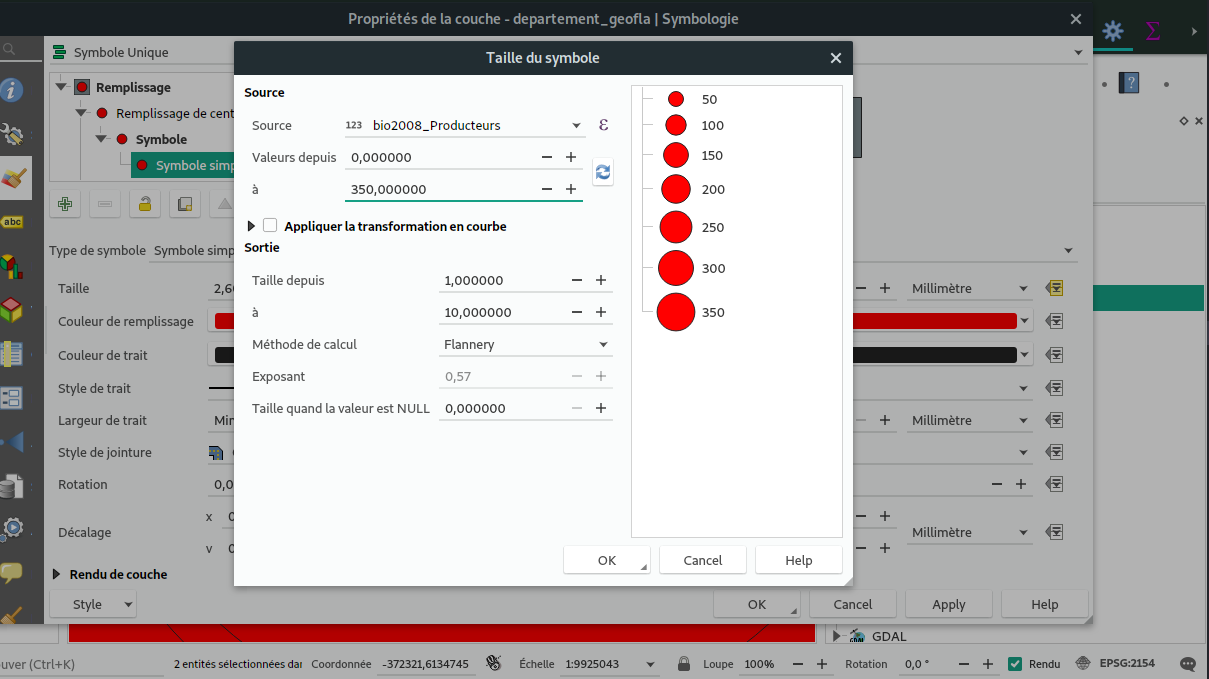
\includegraphics[width=0.9\textwidth]{img/symbolesProp.png}\label{fig:symbolesProp}}\\
  \subfigure[]{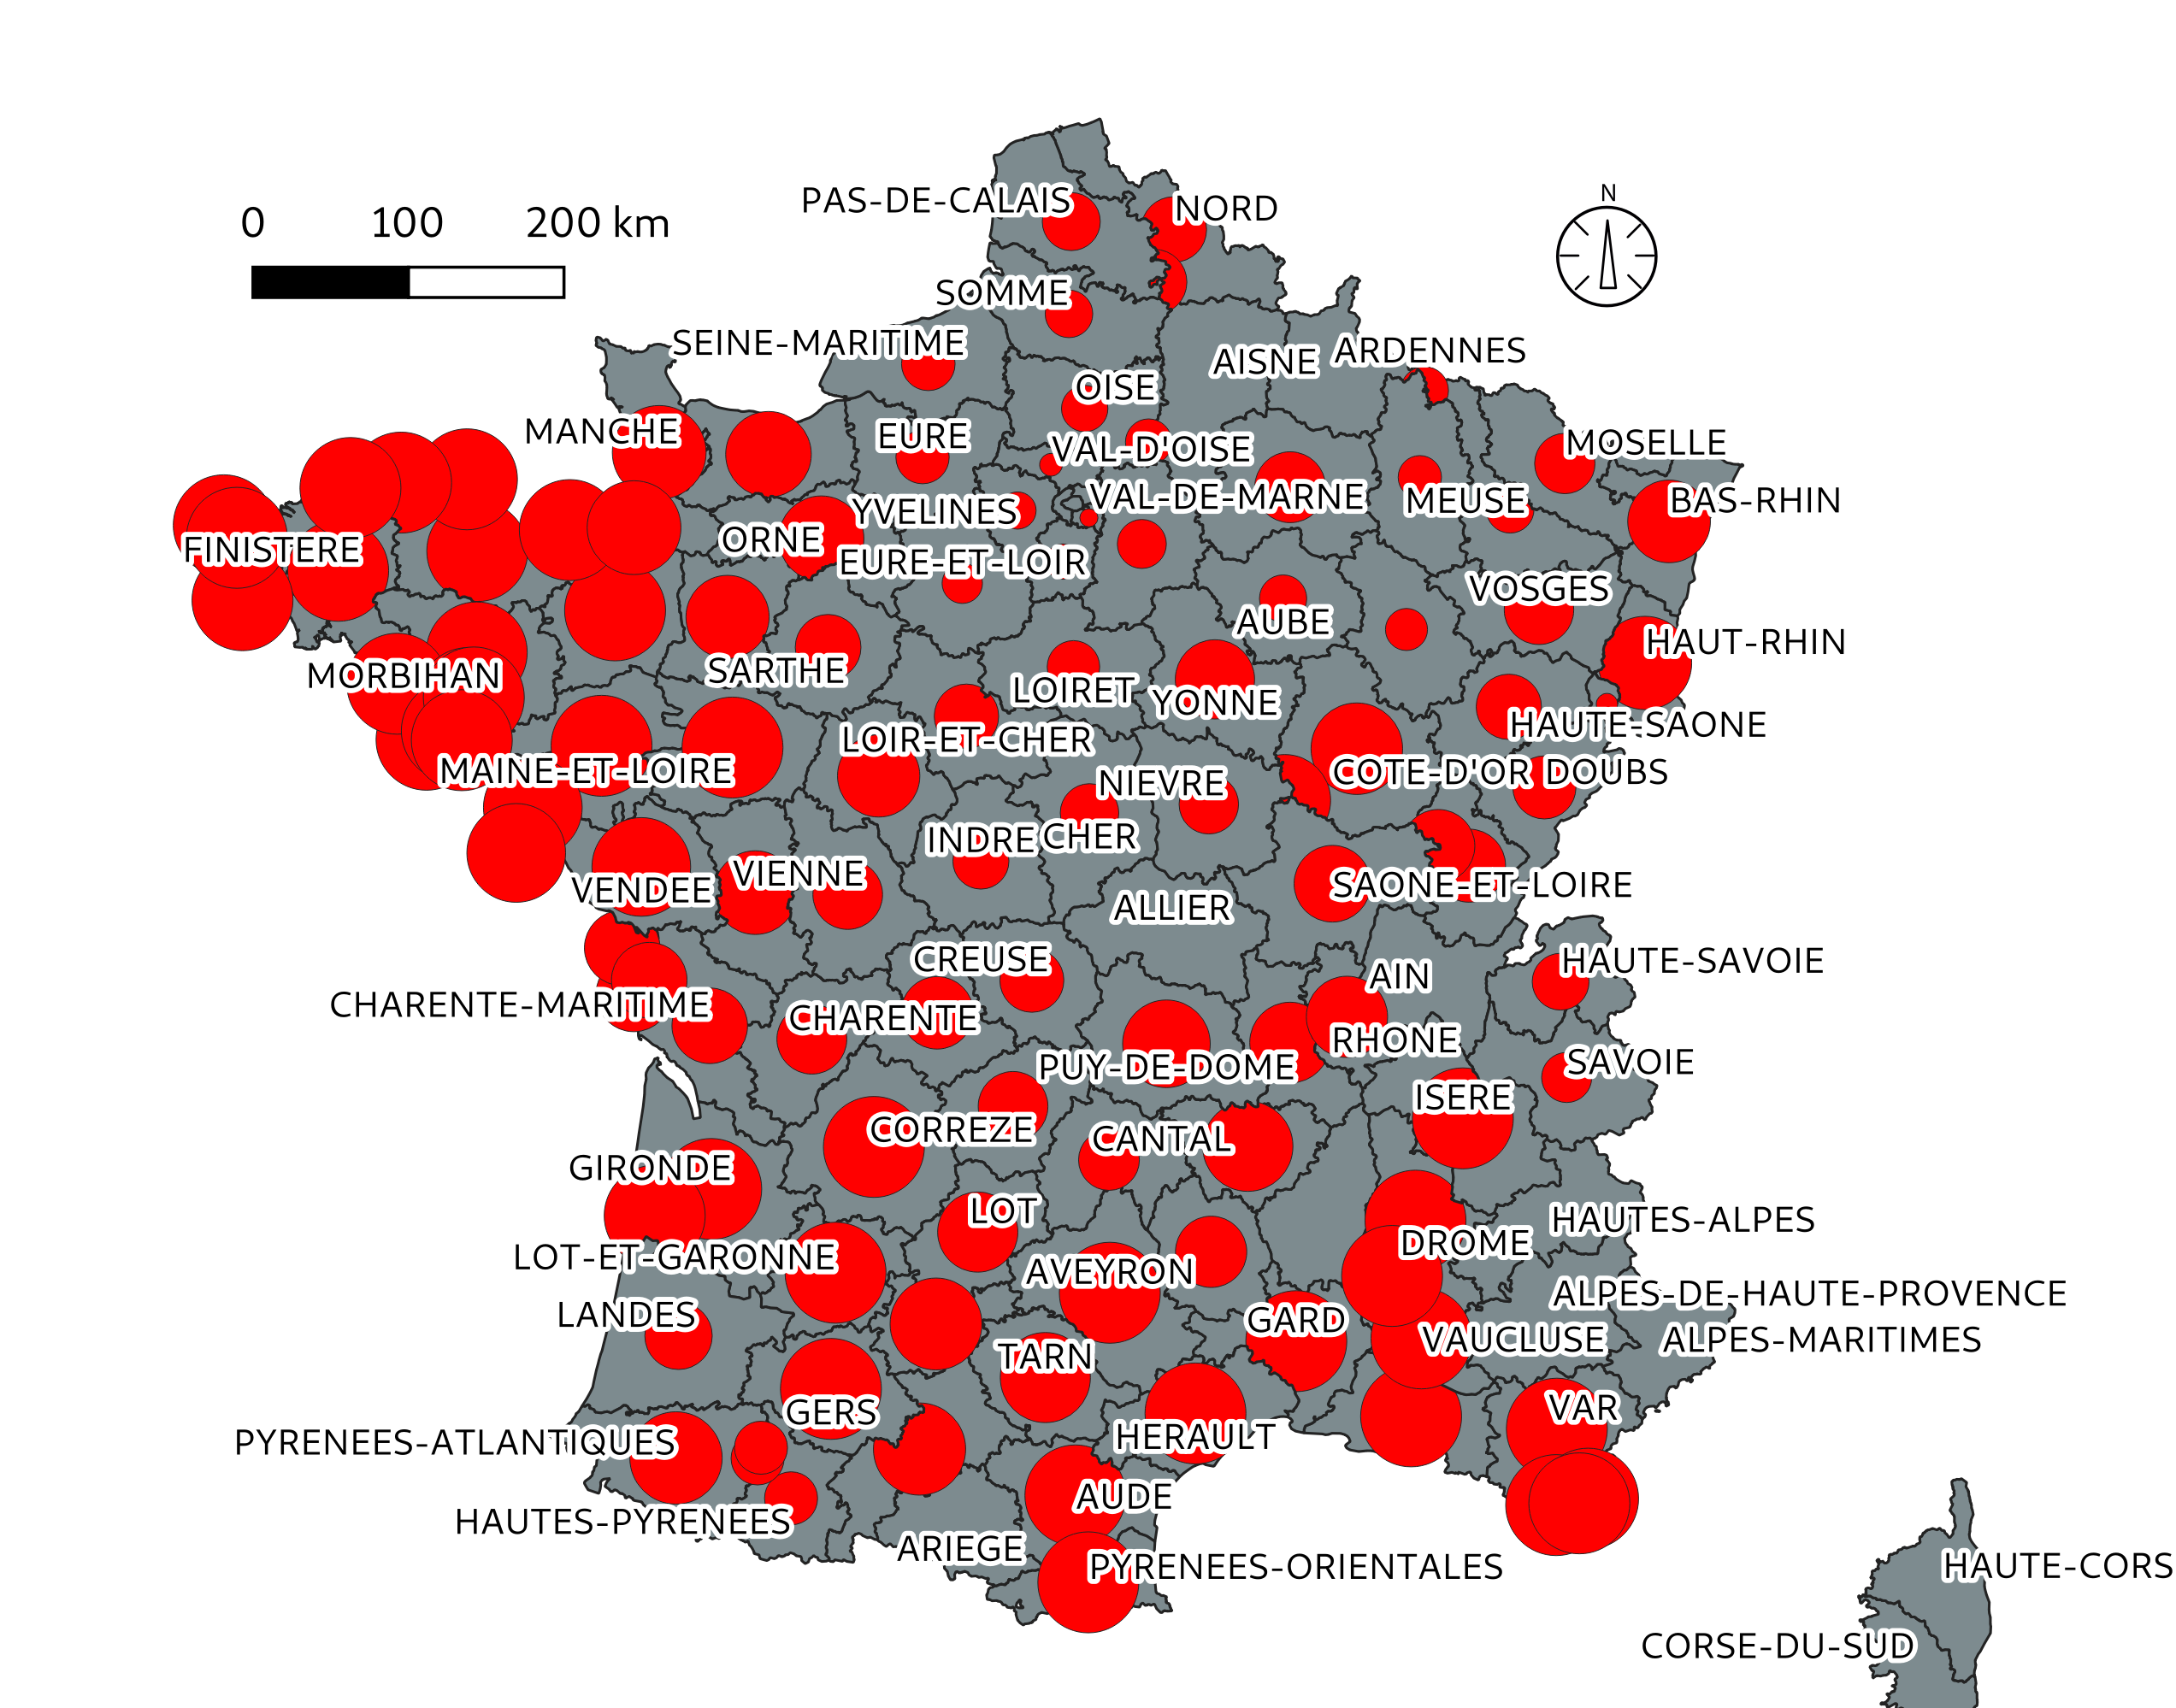
\includegraphics[width=0.9\textwidth]{img/carte_france2.png}\label{fig:carte_symbole}}
    \caption{Des symboles proportionnels}\label{fig:analyseThematique}
  \end{figure}

\section{Traitements à partir de rasters}
  Qgis est capable de travail sur des images raster grâce à un certain nombre de librairies qui sont embarquées. Nous allons ici effectuer quelques traitements à partir de données altitudinales.

  Mettons-nous en situation. Vous travaillez dans un bureau d'études spécialisé dans les études d'impact environnemental. Un client vous a missionné pour implanter une éolienne sur un territoire.

  Vous n'avez pas beaucoup d'argent, vous allez donc essayer de vous débrouiller avec des données libres et gratuites ! La première chose à faire est de télécharger un modèle numérique de terrain (MNT ou DTM digital Terrain Model en anglais). Par chance, la mission SRTM propose gratuitement des données de MNT pour le monde entier avec une résolution de 90 mètres.

  Vous pouvez les télécharger sur le site \url{http://srtm.csi.cgiar.org/,} mais je vous ai téléchargé les tuiles pour le Limousin dans le fichier de données (\texttt{srtm\_37\_03} et \texttt{srtm\_37\_04}).

  \subsection{Prépéarer la donnée}

  Vous pouvez ouvrir les tuiles sur Qgis et vous constaterez qu'elles sont en projection WGS84. Or, nous travaillons en France en projection Lambert 93. Vous constatez aussi que le Limousin est à cheval sur deux tuiles (surtout le sud de la Corrèze). Le premier travail va donc consister à assembler les deux raster, les reprojeter en Lambert 93 et les découper en suivant les contours du Limousin.

    \subsubsection{Assembler des raster}

    Vous avez chargé les deux raster dans Qgis (même méthode que dans la section \ref{part:chargerData}). Pour les assembler de manière efficace, sans pour autant prendre de la place sur le disque dur, et faciliter le chargement (que des avantages !), on peut créer un raster virtuel (dans le menu Raster -> Divers -> construire un raster virtuelraster virtuel).

    Après avoir choisi les raster en entrée et les méthodes d'échantillonnage si les raster avaient des résolutions différentes vous pouvez enregistrer le raster virtuel dans un fichier ou le garder en cache pour un travail temporaire dans Qgis.

    Astuce : Vous noterez que la construction d'un raster virtuel utilise une fonction de la librairie gdal. Chaque fois que vous renseignez un champ, la partie texte s'allonge et vous permet de voir comment se constitue cette fonction gdalbuildvrt (fig. \ref{fig:buildvr}).

    \subsubsection{Reprojeter des raster}

    Le raster virtuel se comporte comme un raster normal, tandis que si vous allez dans le dossier où vous l'avez créé, vous constaterez que ce n'est qu'un fichier texte qui permet à Qgis d'assembler mécaniquement les deux rasters, et de les considérer comme une seule entité.

    Ce raster est toujours en projection WGS84, et nous voudrions le reprojeter en Lambert 93. Pour cela vous allez utiliser l'outil reprojectionreprojection qui se trouve dans le menu Raster-> Projections -> Projection).

    Vous avez plusieurs rasters ouverts, il faudra choisir dans le menu les rasters à reprojeter, s'il n'y en a qu'un, il sera disponible immédiatement. Vous allez devoir définir la projection en entrée (SRC Source), avec Sélections vous pouvez partir à la recherche de la projection WGS84.

    Vous spécifiez la projection en sortie (SRC sortie) et vous sélectionnez, de la même manière que pour l'entrée, la projection Lambert 93 (EPSG:2154\footnote{EPSG pour \textit{European Petroleum Survey Group}, défini une liste des systèmes de coordonnées géoréférencées et leur a associé des codes pour les identifier. Ces codes sont notamment utilisés dans les standards de l'Open Geospatial Consortium}).

    Si vous avez plusieurs cœurs sur votre ordinateur, et que le raster est pesant, vous pouvez envoyer l'action en multithread et valider

    \begin{figure}
    \centering
    \subfigure[]{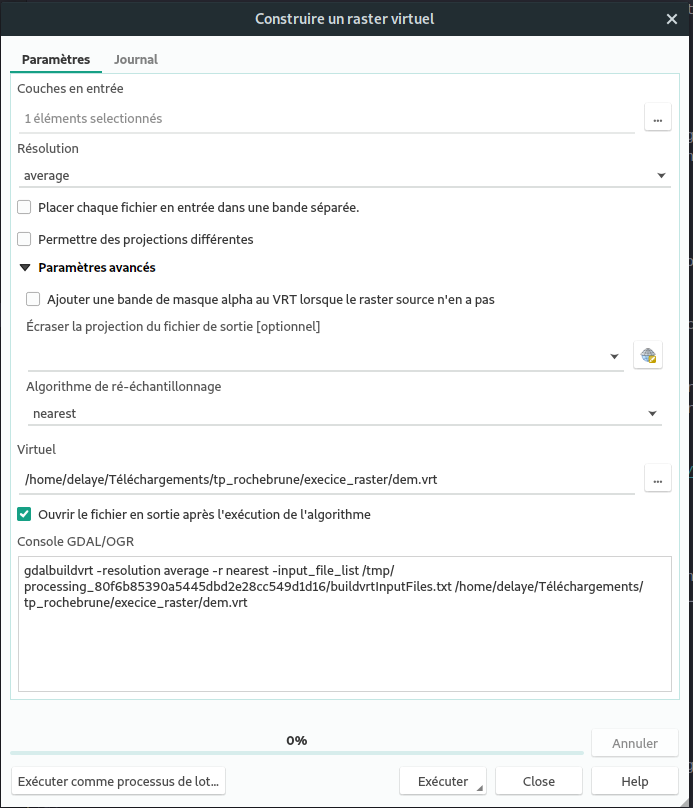
\includegraphics[width=0.9\textwidth]{img/bd_gdalbuildvr}\label{fig:buildvr}}\\
    \subfigure[]{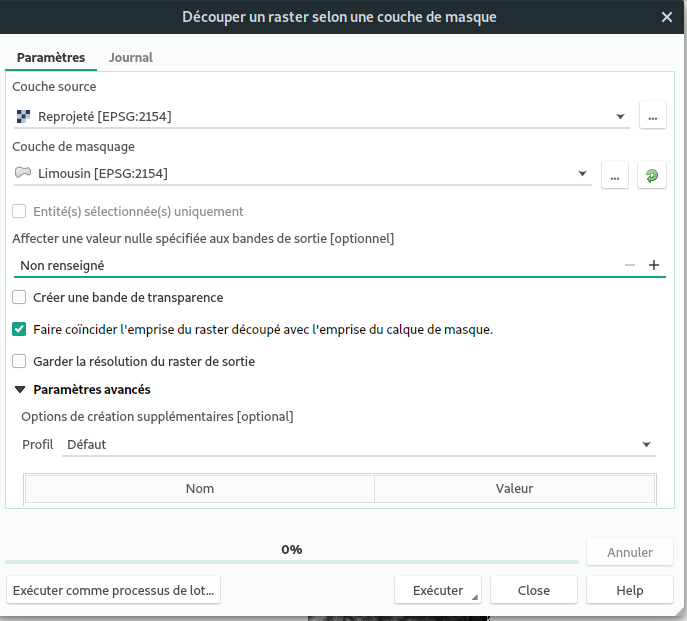
\includegraphics[width=0.9\textwidth]{img/bd_decoupeRaster}\label{fig:decoupraster}}
      \caption{Des symboles proportionnels}\label{fig:analyseThematique}
    \end{figure}

    \subsubsection{Découper le raster en fonction d’un polygone}

    Vous avez maintenant besoin d'ouvrir la couche polygone du Limousin que je vous ai préparée en plus d'un raster reprojeté. La découpe du raster en fonction d'un polygone se fait dans le menu Raster -> Extraction -> Découper une raster selon une couche de masque) .

    Sélectionner le raster en entrée, le raster en sortie. Vous pouvez ensuite sélectionner la découpe du raster avec une emprise rectangulaire (en fournissant les coordonnées) ou avec une couche de masquage (fig. \ref{fig:decoupraster}).

    Nous allons effectuer la seconde solution (couche de masquage) avec la couche de polygone Limousin. Ensuite, validez et vous obtenez en sortie une belle découpe bien projetée (fig. \ref{fig:carte_limousin_decoup})!

    \begin{figure}
    \centering
    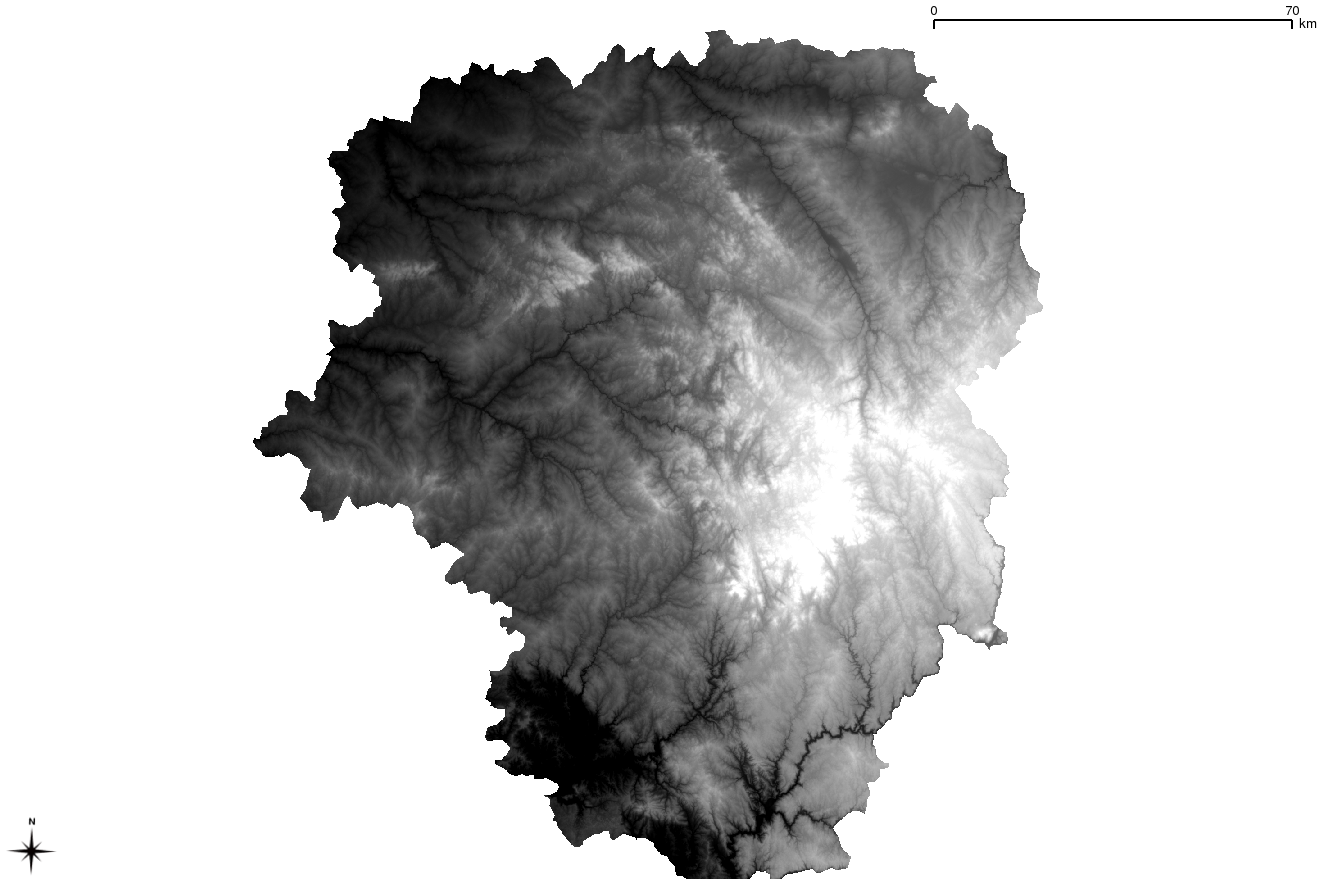
\includegraphics[width=0.9\textwidth]{img/rasterLimousin}
      \caption{Raster découper selon un polygone}\label{fig:carte_limousin_decoup}
    \end{figure}

    \subsubsection{Calcul sur rasters : exemple de co-visibilité}

    Je vous ai préparé également un dossier shapefile qui contient un point pour situer la zone d'implantation éolienne. Vous devez avoir ouvert maintenant dans Qgis le Limousin, et le point nommé héol.shp .

    Il existe plusieurs solutions pour faire des calculs de covisibilité dans Qgis. On peut utiliser GRASS-GIS en tant qu'extension et on peut aussi utiliser GRASS-GIS ou SAGA-GIS dans Sextante (depuis la version 2.0.X). Comme nous travaillons sur la version 3, nous allons utiliser les outils Sextante. Pour les activer, accédez au menu Traitement -> boite à outils, faisant apparaitre une boite à outils sur la droite de l'interface. Vous chercherez la fonction \texttt{r.viewshed} .

    Renseignez ensuite sur quelle couche de MNT l'algorithme va calculer,  la position du champ d'éoliennes, la taille de l'objet (ici nos éoliennes), j'ai choisi 20m, la distance maximum à laquelle on peut voir l'objet (constater une nuisance), enfin la résolution à laquelle va travailler GRASS.

    Vous pouvez sauvegarder le résultat sous forme d'un raster ou simplement le garder en mémoire tampon.

    Vous n'avez plus qu'à faire tourner l'algorithme... pour produire la figure \ref{fig:carte_limousin_covisibilite}

    \begin{figure}
    \centering
    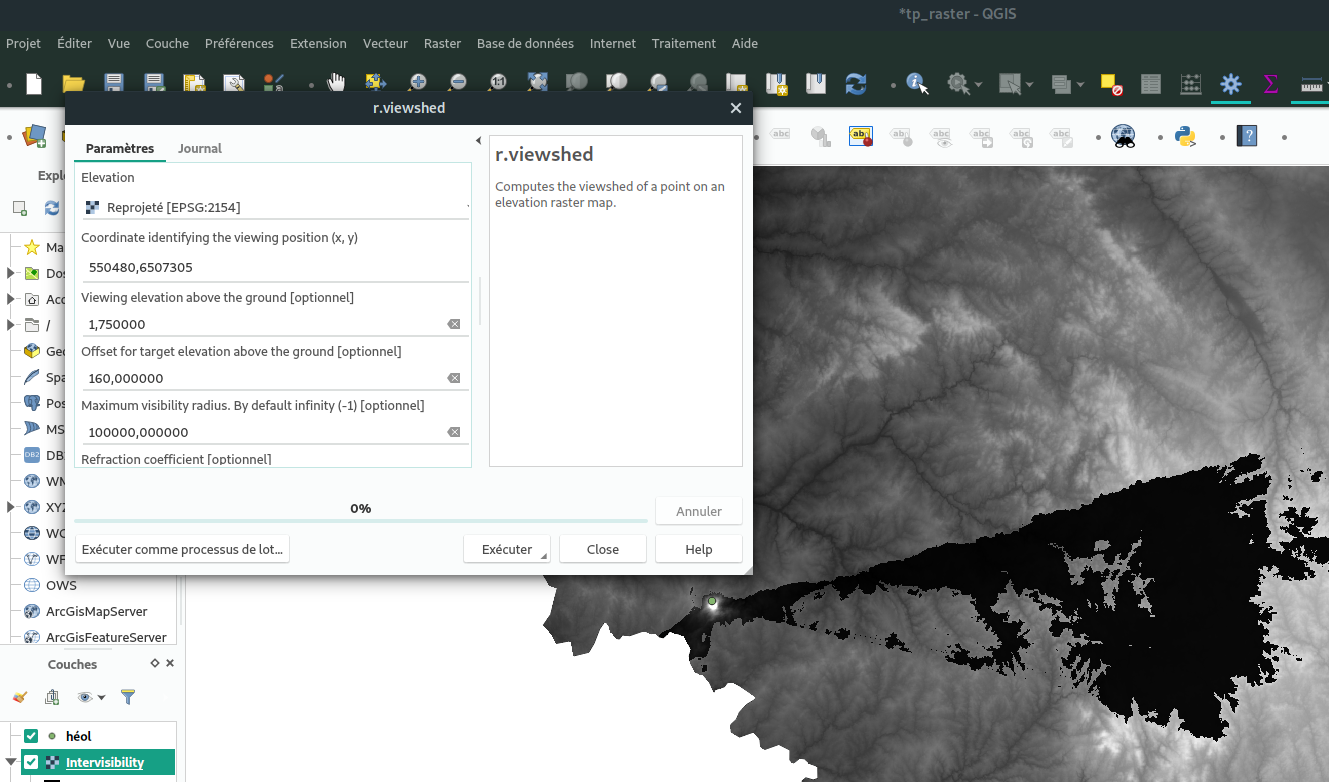
\includegraphics[width=0.9\textwidth]{img/rViewshed}
      \caption{Carte de covisibilité}\label{fig:carte_limousin_covisibilite}
    \end{figure}

    Attention ce calcul ne tient compte que du relief. Si nous voulions tenir compte de la forêt (ce qui serait intéressant), il aurait fallu découper les zones boisées à partir d'Openstreetmap ou de données Corine land cover, les transformer en raster et ajouter 4 à 5 mètres au MNT à toutes les zones boisées...


\end{document}
